\documentclass[a4paper, 14pt]{extarticle}

% Поля
%--------------------------------------
\usepackage{geometry}
\geometry{a4paper,tmargin=2cm,bmargin=2cm,lmargin=3cm,rmargin=1cm}
%--------------------------------------


%Russian-specific packages
%--------------------------------------
\usepackage[T2A]{fontenc}
\usepackage[utf8]{inputenc} 
\usepackage[english, main=russian]{babel}
%--------------------------------------

\usepackage{textcomp}

% Красная строка
%--------------------------------------
\usepackage{indentfirst}               
%--------------------------------------             


%Graphics
%--------------------------------------
\usepackage{graphicx}
\graphicspath{ {./images/} }
\usepackage{wrapfig}
%--------------------------------------

% Полуторный интервал
%--------------------------------------
\linespread{1.3}                    
%--------------------------------------

%Выравнивание и переносы
%--------------------------------------
% Избавляемся от переполнений
\sloppy
% Запрещаем разрыв страницы после первой строки абзаца
\clubpenalty=10000
% Запрещаем разрыв страницы после последней строки абзаца
\widowpenalty=10000
%--------------------------------------

%Списки
\usepackage{enumitem}

%Подписи
\usepackage{caption} 

%Гиперссылки
\usepackage{hyperref}

\hypersetup {
	unicode=true
}

%Рисунки
%--------------------------------------
\DeclareCaptionLabelSeparator*{emdash}{~--- }
\captionsetup[figure]{labelsep=emdash,font=onehalfspacing,position=bottom}
%--------------------------------------

\usepackage{tempora}
\usepackage{amsmath}
\usepackage{color}
\usepackage{listings}
\lstset{
  belowcaptionskip=1\baselineskip,
  breaklines=true,
  frame=L,
  xleftmargin=\parindent,
  language=Java,
  showstringspaces=false,
  basicstyle=\footnotesize\ttfamily,
  keywordstyle=\bfseries\color{blue},
  commentstyle=\itshape\color{purple},
  identifierstyle=\color{black},
  stringstyle=\color{red},
}

%--------------------------------------
%			НАЧАЛО ДОКУМЕНТА
%--------------------------------------

\begin{document}

%--------------------------------------
%			ТИТУЛЬНЫЙ ЛИСТ
%--------------------------------------
\begin{titlepage}
\thispagestyle{empty}
\newpage


%Шапка титульного листа
%--------------------------------------
\vspace*{-60pt}
\hspace{-65pt}
\begin{minipage}{0.3\textwidth}
\hspace*{-20pt}\centering

\includegraphics[width=\textwidth]{emblem}
\end{minipage}
\begin{minipage}{0.67\textwidth}\small \textbf{
\vspace*{-0.7ex}
\hspace*{-6pt}\centerline{Министерство науки и высшего образования Российской Федерации}
\vspace*{-0.7ex}
\centerline{Федеральное государственное бюджетное образовательное учреждение }
\vspace*{-0.7ex}
\centerline{высшего образования}
\vspace*{-0.7ex}
\centerline{<<Московский государственный технический университет}
\vspace*{-0.7ex}
\centerline{имени Н.Э. Баумана}
\vspace*{-0.7ex}
\centerline{(национальный исследовательский университет)>>}
\vspace*{-0.7ex}
\centerline{(МГТУ им. Н.Э. Баумана)}}
\end{minipage}
%--------------------------------------

%Полосы
%--------------------------------------
\vspace{-25pt}
\hspace{-35pt}\rule{\textwidth}{2.3pt}

\vspace*{-20.3pt}
\hspace{-35pt}\rule{\textwidth}{0.4pt}
%--------------------------------------

\vspace{1.5ex}
\hspace{-35pt} \noindent \small ФАКУЛЬТЕТ\hspace{80pt} <<Информатика и системы управления>>

\vspace*{-16pt}
\hspace{47pt}\rule{0.83\textwidth}{0.4pt}

\vspace{0.5ex}
\hspace{-35pt} \noindent \small КАФЕДРА\hspace{50pt} <<Теоретическая информатика и компьютерные технологии>>

\vspace*{-16pt}
\hspace{30pt}\rule{0.866\textwidth}{0.4pt}
  
\vspace{11em}

\begin{center}
\Large {\bf Летучка № 1} \\ 
\large {\bf по курсу <<Языки и методы программирования>>} \\ 
\large <<Установка Java на VDS сервер и запуск веб-серверов>>
\end{center}\normalsize

\vspace{8em}


\begin{flushright}
  {Студент группы ИУ9-21Б Воронков А. С.\hspace*{15pt} \\
  \vspace{2ex}
  Преподаватель Посевин Д. П.\hspace*{15pt}}
\end{flushright}

\bigskip

\vfill
 

\begin{center}
\textsl{Москва 2026}
\end{center}
\end{titlepage}
%--------------------------------------
%		КОНЕЦ ТИТУЛЬНОГО ЛИСТА
%--------------------------------------

\renewcommand{\ttdefault}{pcr}

\setlength{\tabcolsep}{3pt}
\newpage
\setcounter{page}{2}

\section{Цель}\label{Sect::task}
\par
Создать учетную запись на VDS сервере, установить на него Java, скомпилировать и запустить две версии веб-сервера.
\pagebreak
\section{Практическая реализация}
Код файла HttpServer.java
\begin{lstlisting}
import java.io.BufferedReader;
import java.io.IOException;
import java.io.InputStreamReader;
import java.io.PrintWriter;
import java.net.ServerSocket;
import java.net.Socket;
import java.nio.charset.StandardCharsets;

public class HttpServer {

    public static void main(String[] args) {
        try (ServerSocket serverSocket = new ServerSocket(5678)) {
            System.out.println("Server started!");
            
            while (true) {
                // ожидаем подключения
                Socket socket = serverSocket.accept();
                System.out.println("Client connected!");

                // для подключившегося клиента открываем потоки 
                // чтения и записи
                try (BufferedReader input = new BufferedReader(new InputStreamReader(socket.getInputStream(), StandardCharsets.UTF_8));
                     PrintWriter output = new PrintWriter(socket.getOutputStream())) {

                    // ждем первой строки запроса
                    while (!input.ready()) ;

                    // считываем и печатаем все что было отправлено клиентом
                    System.out.println();
                    while (input.ready()) {
                        System.out.println(input.readLine());
                    }

                    // отправляем ответ
                    output.println("HTTP/1.1 200 OK");
                    output.println("Content-Type: text/html; charset=utf-8");
                    output.println();
                    output.println("<p>Привет всем!</p>");
                    output.flush();
                    
                    // по окончанию выполнения блока try-with-resources потоки, 
                    // а вместе с ними и соединение будут закрыты
                    System.out.println("Client disconnected!");
                }
            }
        } catch (IOException ex) {
            ex.printStackTrace();
        }
    }
}
\end{lstlisting}
\par
Код файла Test.java
\begin{lstlisting}
import java.io.IOException;
import java.io.OutputStream;
import java.net.InetSocketAddress;

import com.sun.net.httpserver.HttpExchange;
import com.sun.net.httpserver.HttpHandler;
import com.sun.net.httpserver.HttpServer;

public class Test {

    public static void main(String[] args) throws Exception {
        HttpServer server = HttpServer.create(new InetSocketAddress(5678), 0);
        server.createContext("/test", new MyHandler());
        server.setExecutor(null); // creates a default executor
        server.start();
    }

    static class MyHandler implements HttpHandler {
        @Override
        public void handle(HttpExchange t) throws IOException {
            String response = "This is the response";
            t.sendResponseHeaders(200, response.length());
            OutputStream os = t.getResponseBody();
            os.write(response.getBytes());
            os.close();
        }
    }
}
\end{lstlisting}

\section{Результаты}
В результате работы программы получилось запустить веб-сервер с отображением сообщения "Всем привет!" и веб сервер с отображением сообщения "This is the response".

\begin{center}
    \nopagebreak
    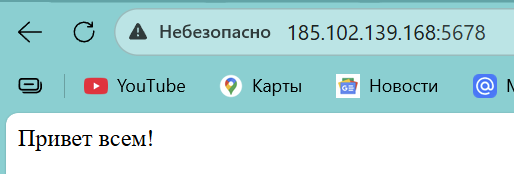
\includegraphics[width=0.85\textwidth]{serv1}
    \captionof{figure}{Веб-сервер 1}
    \vspace{1.5em} 

    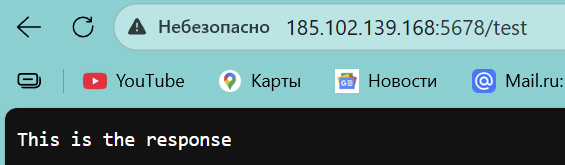
\includegraphics[width=0.85\textwidth]{serv2}
    \captionof{figure}{Веб-сервер 2}
    \vspace{1.5em}
\end{center}

\section{Вывод}
В данной лабораторной работе были получены минимальные навыки работы с VDS сервером. Была произведена подготовка к работе с Java на сервере в дальнейшем. Был произведен тестовый запуск двух простейших веб-серверов.
\end{document}